% ------------------------------------------------
% Page start
% ------------------------------------------------
\chapter{Table design}
\label{chapter:table_design}

\baselineskip=26pt
\thispagestyle{empty}
% ------------------------------------------------

The target of Li's Hash is to provide a similar usage of relational database to user who can use the non-relational database as the back-end, so that the table design in relational database is needed in Li's Hash. By combining the data type which has introduced before that can become a table which the concept is show as figure \ref{fig:table_design:example}:

\begin{figure}[h]
\centering
%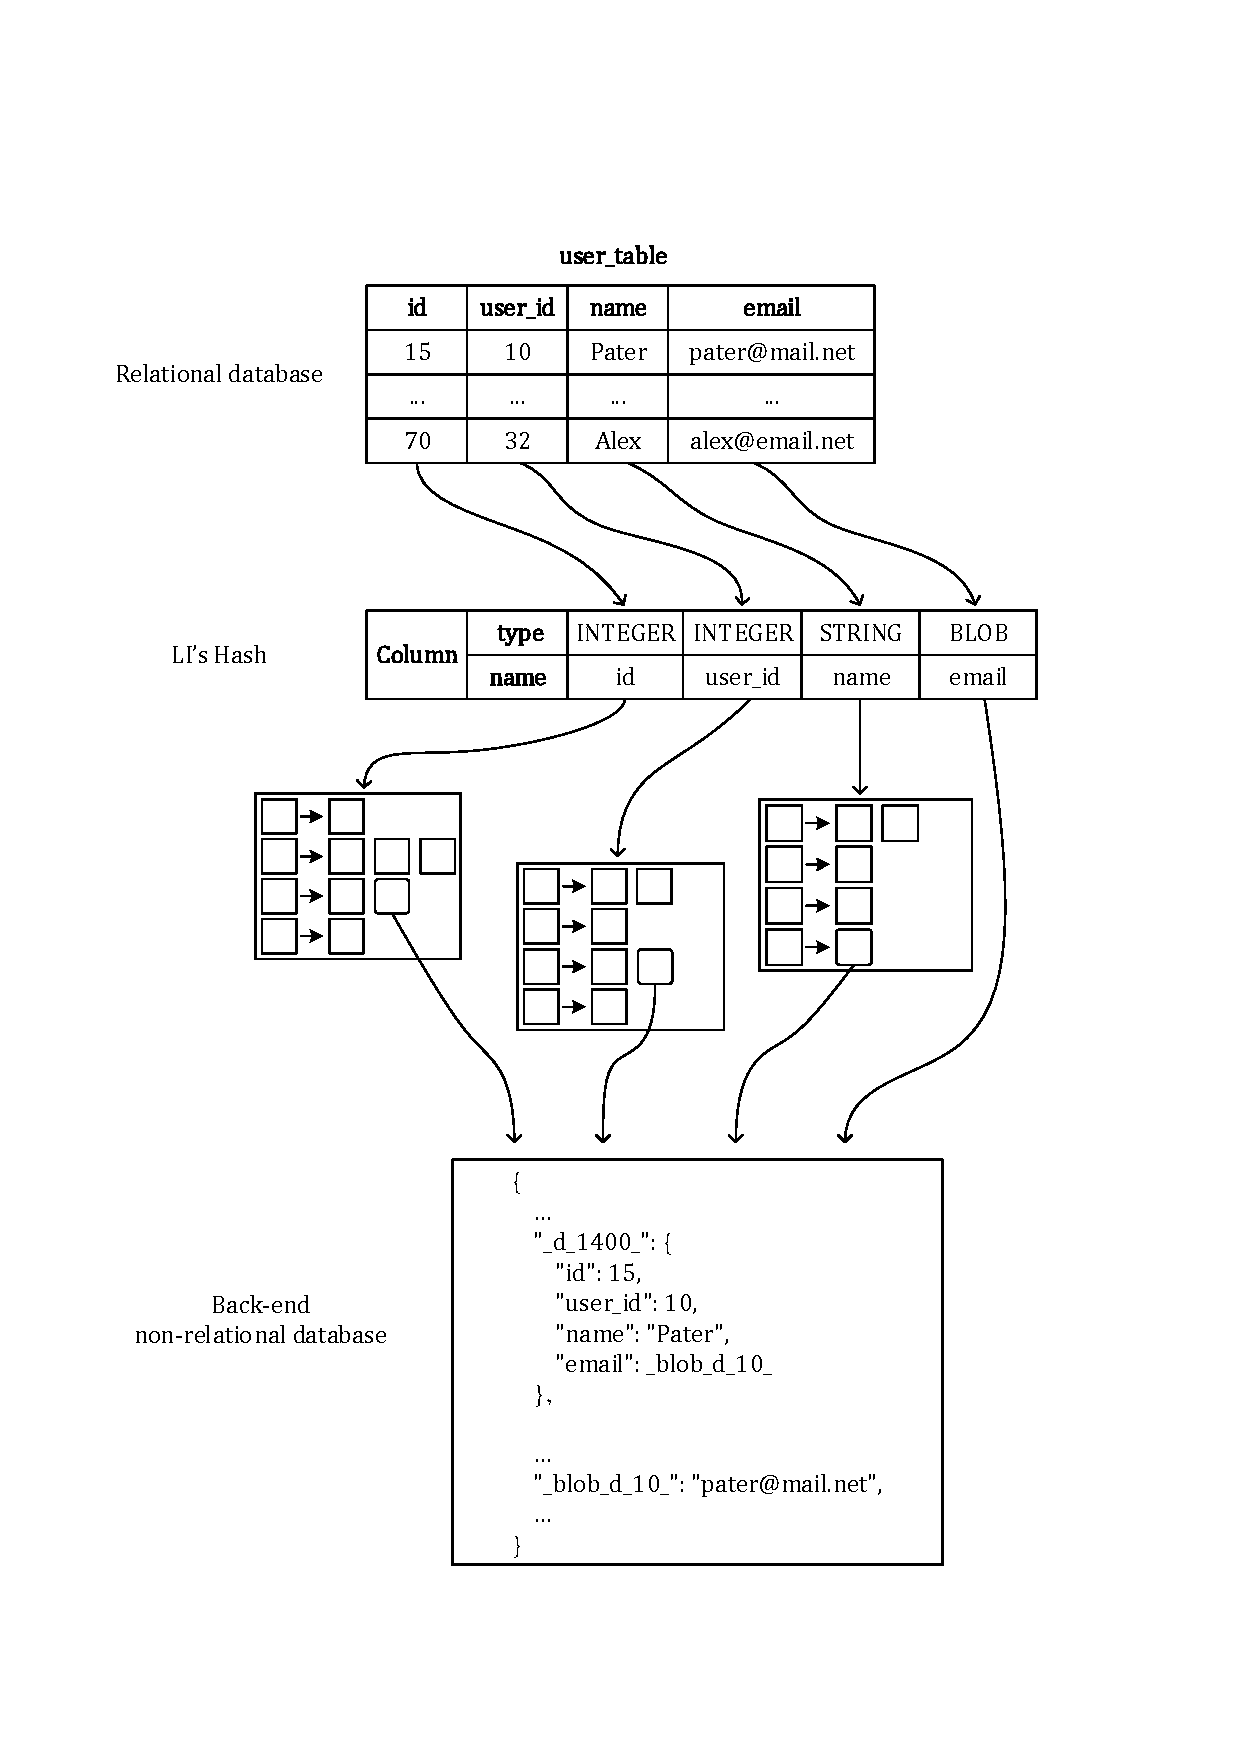
\includegraphics[scale=0.7]{./table-design/pic/design_example_v2.pdf}
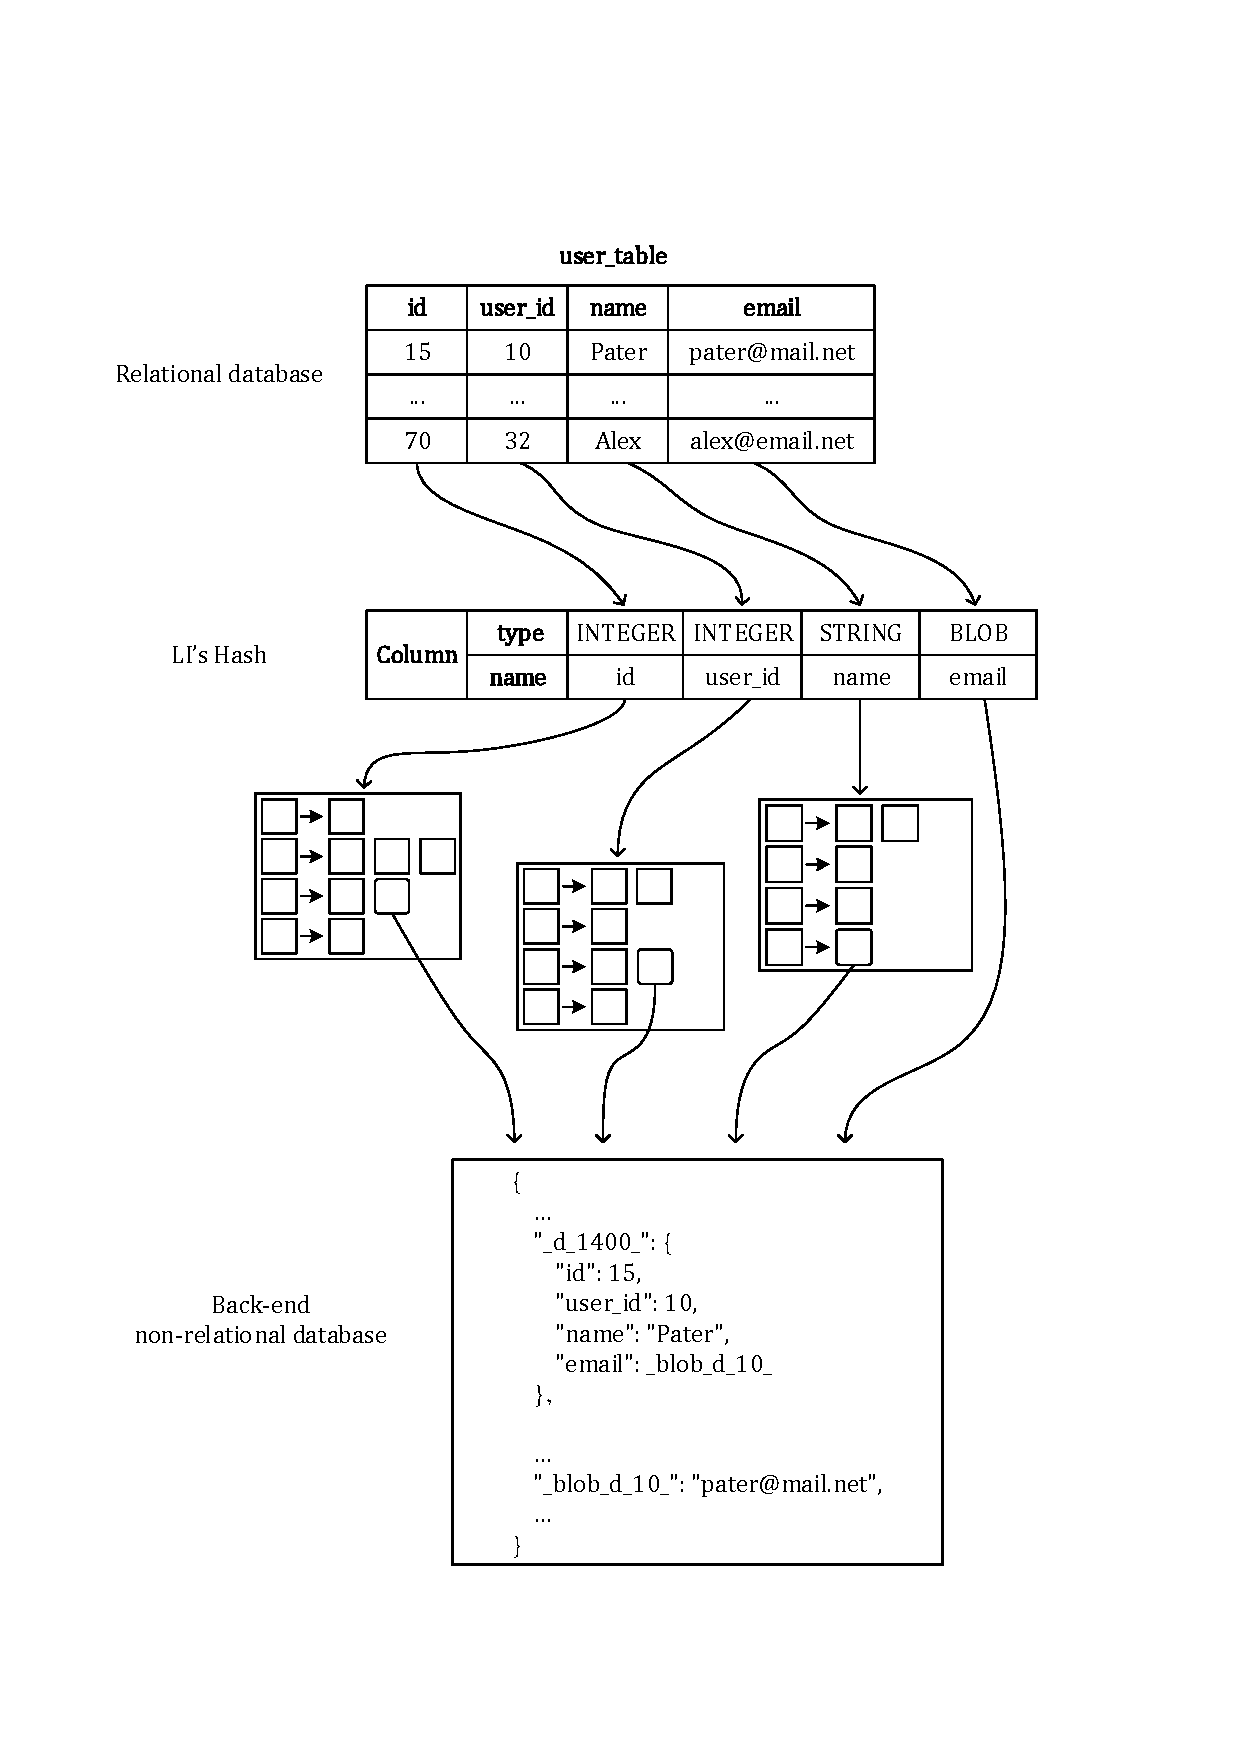
\includegraphics[width=0.6\textwidth]{./table-design/pic/design_example_v2.pdf}
\caption{The view on each layer.}
\label{fig:table_design:example}
\end{figure}

Figure \ref{fig:table_design:example} shows a example of simple membership data-base, the user who using the Li's Hash that will see the view as a normal relational database, but the table is builded by the Li's Hash which do the indexing and store all data into the back-end database just like figure shows.\\

%This is the target that the Li's Hash want to provide for the users.

%table for the user, from the relational databases design \cite{web:mysql:sql-syntax-identifiers,web:sqlite:limits,web:postgresql:sql-syntax-identifiers} which seem normally to set the maximum length of table and column name as 63~64 or no limited. So the maximum length should be 255 for the names which should enough for many user, also plus the length of database's name (for application that multiuser using a single backend database) and the key's length (255 as the other non-relational databases), it should be at least 1000,

\clearpage

% ------------------------------------------------
% End of page
% ------------------------------------------------
